\documentclass[class=book, crop=false]{standalone}
\usepackage[subpreambles=true]{standalone}
\usepackage{/home/mark/Documents/gradschool/research/thesis/preamble}
\usepackage{import}

\begin{document}

\chapter{Exceptional Cases}
\label{exceptional}
In the previous chapter we were able to show that $U_+$ is not finitely generated for a large family of Coxeter groups $W$ with labels $a\le b\le c.$ These results were based on assuming $b\ge 4$ which allowed us to show that $\D$ was infinite and proceed from there. In fact, we didn't even describe all of the chambers in $\D,$ just an infinite family. However, the same approach will not work in the remaining cases because of the following lemma.
\begin{lemma} If $W$ is a Coxeter group with labels $a\le b\le c$ as before, then $\D=\alpha_1\cap \alpha_n\cap \beta\cap \beta'$ as defined in the previous chapter is infinite if and only if $b\ge 4.$
	\label{lem:infD}
\end{lemma}
\begin{proof}
	We know by Lemma \ref{lem:infmany} that $\D$ is infinite if $b\ge 4.$ Thus it remains to show that $\D$ is finite if $b=3.$ If $b=3$ then $a=3$ also, and by definition of $a,b,c$ this means $m(s,t)=m(s,u)=3.$ We will also recall the definition of $\D=\alpha_1\cap \alpha_n\cap \beta \cap \beta'$ where
	\begin{align*}
	\alpha_1&=\{D\in \Sigma|d(D,C)<d(D,tC)\}=\{w\in W|\ell(w)<\ell(tw)\}\\
	\alpha_n&=\{D\in \Sigma|d(D,C)<d(D,uC)\}=\{w\in W|\ell(w)<\ell(uw)\}\\
	\beta&=\{D\in \Sigma|d(D,tC)<d(D,tsC)\}=\{w\in W|\ell(tw)<\ell(stw)\}\\
	\beta'&=\{D\in \Sigma|d(D,uC)<d(D,usC)\}=\{w\in W|\ell(uw)<\ell(suw)\}
\end{align*}

Let $w\in W$ and suppose $\ell(w)\ge 2.$ Then we can write $w=s_1s_2w'$ where $\ell(w')=\ell(w)-2.$ If $s_1=t$ then we have
\[
	\ell(tw)=\ell(s_2w')=\ell(w)-1<\ell(w)
\]
which shows $w\not\in \alpha_1$ and thus $w\not\in \D.$ A similar argument shows that $w\not\in \D$ if $s_1=u.$

Now we assume $s_1=s$ and so we can also assume $s_2=t,u.$ First let $s_2=t$ so that $w=stw'.$ If $w\not\in \alpha_1$ then $w\not\in \D$ and so we will suppose $w\in\alpha_1.$ Now we can see
\[
	\ell(stw)=\ell(ststw')=\ell(sstsw')=\ell(tsw')\le \ell(w')+2=\ell(w)<\ell(tw)
\]
and thus $w\not\in \D.$ A similar argument shows that $w\not\in \D$ if $s_2=u.$

We have shown that if $\ell(w)\ge 2$ then $w\not\in \D$ and thus $\D$ must be finite as desired. In fact, if $a=b=3$ then we can check relatively easily that $\D=\{C,sC\}$ which proves the desired result.
\end{proof}

The previous lemma shows that generating results for the remaining cases is not just a matter of being slightly more clever when we look for vertices, but changing the strategy as a whole. In fact, in some cases our proof strategy needs to switch entirely since $U_+$ will be finitely generated in some cases as we will see. First, we will show which of the remaining cases are not finitely generated.

All of the remaining rank 3 cases have the property that $m(s,u)=m(s,t)=3.$ If $x$ is the vertex of $C$ of type $s$ then $x$ is the only possible vertex of type $C$ with the property that $[U_x:U'_x]\ge 2.$ With two edge labels of $3$ it is impossible for $U_x\cong {}^2F_4(2)$ and so the only remaining possibilites are $U_x\cong C_2(2),G_2(2),$ and $G_2(3).$ We will enumerate through each of these cases individually.

\section{Case: $U_x\cong G_2(2)$}
We saw in the previous chapter that a vertex contained in $\D$ was a sufficient condition to construct a corresponding map $\tilde{\phi_v}.$ However, it is not a necessary condition, and we will see in this section we can relax a few conditions to still construct $\tilde{\phi_v}$ for infinitely many vertices. Our first step is to make some general observations about this case and then prove a statment similar to Lemma \ref{lem:existence}.

For the remainder of the section we will assume that $(G,(U_\alpha)_{\alpha\in \Phi},T)$ is an RGD system of type $(W,S)$ where $S=\{s,t,u\}$ and 
\[
	W=\langle s,t,u|s^2=t^2=u^2=(st)^3=(su)^3=(tu)^6=1\rangle
\]
Furthermore, let $x$ be the vertex of $C$ of type $s$ and assume that $U_x\cong G_2(2).$ Recall that this means $[U_x:U'_x]=4$ and $[U_v:U'_v]=4$ for all vertices $v$ of type $s$ by Lemma \ref{lem:index} and Lemma \ref{lem:resporder}.

Recalling from the previous chapter, we know that there is a presentation of $U_+$ generated by $U_\alpha$ for all $\alpha\in \Phi_+.$ Again, there are several types of relations we need to consider. There are relations among the $U_\alpha$ and there are relations between $U_\alpha$ and $U_\beta$ when $\{\alpha,\beta\}$ is a prenilpotent pair. By \eqref{assume} we know that $[U_\alpha,U_\beta]=\{1\}$ if $\alpha$ and $\beta$ are nested. We also know that when $\partial\alpha\cap \partial\beta\neq \emptyset$ that $[u,u']=w$ for some word $w\in U_{(\alpha,\beta)}$ where $u\in U_\alpha$ and $u'\in U_\beta.$ 

Now recall from Chapter \ref{ch:known} that there is a surjective homormorphism $\phi_x:U_x\to H$ where $H$ is a cyclic group. We can also choosea standard labeling $\alpha_1,\dots,\alpha_6$ of the positive roots through $x$ in such a way that $\ker \phi_x=U''_x=\langle U_1,U_5,U_6\rangle.$ Similarly to the last chapter, if $v$ is any vertex of type $s,$ our goal is to construct an extension of the form $\tilde{\phi}_v$ in such a way that
\[
	\tilde{\phi}_v(U_\alpha)=\begin{cases}\phi_v(U_\alpha)&v\in \partial\alpha\\
		1&\text{otherwise}\\
\end{cases}
	\]

	If we can do this for enough vertices $v$ then we will be able to show that $U_+$ is not finitely generated in the same way as the previous chapter. Our first step is to prove an analagous result to Lemma \ref{lem:existence} in the current context.

%For any positive root $\alpha$ of $\Sigma,$ we know that $U_\alpha\cong (\F{2},+)$ and thus each $U_\alpha$ is a cyclic group of order 2. This means we can let $u_\alpha$ be the non-identity element of $U_\alpha$ for all $\alpha\in \Phi^+.$ Then we know that $U$ is generated by $\{u_\alpha\}$ for all $\alpha\in \Phi^+$ and there are exactly 3 types of relations:
%\begin{align*}
%	u_\alpha^2&=1&&\text{For all }\alpha\in \Phi^+\\
%[u_\alpha,u_\beta]&=1&&\text{if }\partial\alpha\cap \partial\beta=\emptyset\\
%[u_\alpha,u_\beta]&=w&&\text{where }w\text{ is a word in }U_{(\alpha,\beta)}\subset U_y\text{ where }y=\partial\alpha\cap \partial\beta
%\end{align*}
%Note that is presentation is the same as that in the previous chapter, just slightly simplified since we know precicely which field $k$ we are working with now.
%
%Let $v$ be any vertex of $\Sigma$ of type $s,$ meaning $|\st(v)|=12.$ Then we showed previouly that there is a map $\phi_v:U_v\to K$ where $K$ is a cyclic group of order 2. If we label the positive roots through $v$ as  $\gamma_1,\dots,\gamma_6$ with $\gamma_i\cap \gamma_j\subset \gamma_k$ for $1\le i\le k\le j\le 6,$ then we also know that at least one of $U_{\gamma_2}$ or $U_{\gamma_5}$ must be sent to the identity by $\phi_v.$ By reversal of the numbering, we can assume without loss of generality that $\phi(U_{\gamma_5})=1.$ As in the previous chapter we want to define an extension of $\phi_v$ to a map $\tilde{\phi_v}:U\to K.$ We define this extension by
%\[
%	\tilde{\phi_v}(u_\alpha)=\begin{cases}\phi_v(u_\alpha)&\text{if }v\text{ lies on }\partial\alpha\\1&\text{otherwise}
%	\end{cases}
%	\]
%	Since we have defined $\tilde{\phi_v}$ for all generators, to check it is well defined is a matter of checking the relations in our presentation.To this end we have to following lemma. Again note that this is the same definition as in Lemma \ref{lem:existence}, simply stated in terms of our new, simplified presentation.
%
\begin{lemma} 
	\label{lem:336f2ex}
	Let $v$ be a vertex of $\Sigma$ of type $s,$ meaning $|\st(v)|=12.$ Assume $\gamma_1,\dots,\gamma_6$ is a standard ordering of the positive roots through $v$ such that $U_{\gamma_5}\subset \ker \phi_v.$ If $\gamma_2,\gamma_3,$ and $\gamma_4$ are simple at all other vertices they meet, then $\tilde{\phi_v}$ as defined in Lemma \ref{lem:existence} exists.
\end{lemma}
\begin{proof}
	To check $\tilde{\phi_v}$ is well defined is a matter of checking the relations are satisfied by the images under $\tilde{\phi_v}.$ Since $\tilde{\phi_v}$ has a cyclic group as its codomain, we can see immediately that the first two types of relations will be satisfied regardless of $\alpha$ and $\beta.$ Now to check the third type.

	Suppose $\alpha$ and $\beta$ are any two positive roots with $y=\partial\alpha\cap \partial\beta.$ Then there is a relation in $U_+$ of the form $[u,u']=w$ where $u\in U_\alpha, u'\in U_\beta,$ and $w\in U_{(\alpha,\beta)}.$ Since $[u_\alpha,u_\beta]$ must be mapped to the identity then we just need to check that $w$ is also mapped to the identity. If $y=v$ then $u_\alpha,u_\beta,w$ all lie in $U_v$ and $\tilde{\phi_v}(w)=\phi_v(w)$ which must be the identity because $\phi_v$ is a well defined homomorphism.

	Now suppose $y\neq v.$ Let $\delta_1,\dots,\delta_n$ be the positive roots through $y,$ with a standard labeling, and assume that $\alpha=\delta_i$ and $\beta=\delta_j$ with $i<j.$ There is at most one positive root whose wall can pass through both $v$ and $y,$ call it $\delta_k$ if it exists. If $\delta_k$ does not exist, then no positive roots through $y$ pass through $v$ and so $\tilde{\phi_v}(u_{\delta_m})=1$ for all $m.$ Thus $\tilde{\phi_v}(w)=1$ as desired.

	Now suppose $\delta_k$ does exist and $\delta_k=\gamma_r$ for $r\in \{1,5,6\}.$ Then we know $\tilde{\phi_v}(U_{\delta_m})=\{1\}$ for all  $m\neq k$ and $\tilde{\phi_v}(U_{\delta_k})=\tilde{\phi_v}(U_{\gamma_r})=\phi_v(U_{\gamma_r})=\{1\}$ by the construction of $\phi_v.$ Thus $\tilde{\phi_v}(U_{\delta_m})=\{1\}$ for all $m$ and so $\tilde{\phi_v}(w)=\{1\}$ as well.

	Now suppose $\delta_k$ does exist and $\delta_k=\gamma_r$ for $r\in \{2,3,4\}.$ Then by assumption, $\delta_k$ is simple at $y$ and thus $k=1,n.$ Thus $\tilde{\phi_v}(U_{\delta_m})=\{1\}$ for all $2\le m\le n-1.$ But $w$ is a word in $U_{(\alpha,\beta)}\subset U_{(\delta_2,\delta_{n-1})}$ and thus $\tilde{\phi_v}(w)=1$ again, which gives the result.
\end{proof}

It is worth noting that the hypotheses of this Lemma are weaker than those of Lemma \ref{lem:existence}, and so we have a hope of constructing more $\tilde{\phi_v}$ then the theory of the previous chapter would allow us to. However, many of the ideas will still be similar and the proofs in this section will run parallel to those in the previous chapter.

Let $x$ be the vertex of $C$ of type $s$ as in the previous chapter and let $\alpha_1,\dots,\alpha_6$ be the positive roots through $x,$ labeled as usual. Recall from the previous chapter that
	\begin{align*}
		\alpha_1&=\{D\in \Sigma|d(D,C)<d(D,tC)\}=\{w\in W|\ell(w)<\ell(tw)\}\\
		\alpha_n&=\{D\in \Sigma|d(D,C)<d(D,uC)\}=\{w\in W|\ell(w)<\ell(uw)\}\\
	\beta&=\{D\in \Sigma|d(D,tC)<d(D,tsC)\}=\{w\in W|\ell(tw)<\ell(stw)\}
	\end{align*}
Also assume without loss of generality that $\phi_x(U_{\alpha_5})=\{1\}.$ Now let $\D'=\alpha_1\cap \alpha_6\cap \beta.$ We can now prove a lemma similar to Lemma \ref{lem:containD}.\\
\Huge picture of $\D'$\normalsize\\

\begin{lemma}
	\label{lem:336f2D}
	Let $x$ be the vertex of $C$ of type $s$ so that $|\st(x)|=12.$ Let $\alpha_1,\dots,\alpha_6$ be the positive roots at $x$ with the standard ordering. Also assume that $\phi_x(U_{\gamma_5})=1.$ Suppose $\gamma=\alpha_i$ for $i\in \{2,3,4\}.$ If $\delta$ is any positive root with $\partial\gamma\cap \partial\delta\neq \emptyset$ then $\D'=\alpha_1\cap \alpha_6\cap \beta\subset \gamma\cap \delta$ where 
	\[
	\beta=\{D\in \Sigma|d(D,tC)<d(D,tsC)\}=\{w\in W|\ell(tw)<\ell(stw)\}
	\]
	as in the previous chapter.
\end{lemma}
\begin{proof}
	Since $\gamma$ is a positive root at $x,$ and $\alpha_1,\alpha_6$ are the simple roots at $x,$ we know that $\D'\subset \alpha_1\cap \alpha_6\subset \gamma$ and thus it will suffice to show that $\D'\subset \delta.$

	Let $y=\partial\gamma \cap \partial \delta.$ If $y=x$ then $\delta$ is also a root which passes through $x$ and so $\delta=\alpha_j$ for some $j\neq i.$ Then as before we get $\alpha_1\cap \alpha_6\subset \alpha_j=\delta$ and thus $\mathcal{D}'\subset \delta$ so that $\mathcal{D}'\subset \gamma\cap \delta$ as desired.

	Now suppose that $\partial \gamma\cap \partial \delta=y\neq x.$ From the local geometry of $\Sigma$ around $x$ we can see the following facts. For any $\alpha_i$ with $2\le i\le n-1$ we know that $\partial\alpha_i\cap \alpha_1\cap \alpha_6=\{x\}$ and $\partial\alpha_i\subset \alpha_1\cup\alpha_6.$ Thus the point $y$ will lie in exactly one of $\alpha_1$ or $\alpha_6.$

	First suppose that $y\in \alpha_6$ so that $y\not\in \alpha_1.$ If $\partial\alpha_1\cap \partial\delta=\emptyset$ then there are exactly 3 possibilities. Either $\alpha_1\subset \delta,$ $\delta\subset\alpha_1,$ or $-\delta\subset \alpha_1.$ But the last two possibilites would contradict our assumption that $y\not\in \alpha_1$ and thus we get $\alpha_1\subset \delta$ and thus $\D'\subset \alpha_1\subset \gamma\cap\delta$ as desired.

	Alternatively, assume that $\partial\alpha_1\cap \partial\delta=y'.$ Then the points $x,y,y'$ will form a triangle with sides on walls of $\Sigma.$ Then by the triangle condition, these three vertices must form a chamber, call it $E.$ The points $x,y$ lie on $\partial\gamma=\partial\alpha_i$ and the points $x,y'$ lie on $\partial\alpha_1.$ Since $y$ and $y'$ are adjacent this means that either $\gamma=\alpha_2$ or $\gamma=\alpha_6.$ The latter is a contradiction of our assumptions and thus $\gamma=\alpha_2.$ We know that $y$ and $y'$ are adjacent and $y\in \alpha_6.$ Since neither $y$ or $y'$ lies on $\partial\alpha_6$ this means that $y'\in \alpha_6$ as well.

	We know that $E$ is a chamber in $\st(x)$ with a side on $\partial \alpha_1$ and $\partial\alpha_2.$ let $D=tC$ and $D'$ be the chamber opposite $D$ in $\st(x).$ Then either $E=D$ or $E=D'.$ By definition, $\alpha_1$ is the only wall separating $C$ and $tC$ which means $D=tC\in \alpha_6.$ If $E=D'$ then $D'\in \alpha_6$ since $x,y,y'$ all lie in $\alpha_6.$ But this is a contradiction as $\alpha_6$ cannot contain two opposite chambers in $\st(x).$ Thus $E=D=tC$ and $\delta=\beta$ by definition. Thus $\D'\subset \beta=\delta$ and $\D'\subset \gamma\cap \delta$ as desired.

	If we assume insteach that $y\in\alpha_1$ so that $y\not\in \alpha_6$ then we have the same two possibilites. If $\partial \alpha_6\cap \partial \delta=\emptyset$ then by similar arguments we get $\D'\subset \alpha_6\subset \delta$ and thus $\D'\subset \gamma\cap \delta$ as desired. If $\partial \alpha_6\cap \partial\delta=y'$ then the vertices $x,y,y'$ form a chamber with $y'$ on $\alpha_6.$ Again, by similar arguments as before, this would imply that $\gamma=\alpha_5$ or $\alpha_1,$ both of which are impossible.

	Therefore, regardless of case we have $\D'\subset \gamma\cap \delta$ as desired.
	

\end{proof}
%             I don't think I need this proof any more
%
%The proofs in the previous chapter relied heavily on facts about simple roots, and to aid these proofs we had Lemma \ref{preservesimple} which shows the $W$ action on $\Sigma$ preserves simplicity under certain condidtions. Now that we are dealing more than just simple roots we need to extend this lemma to the current context.
%
%\begin{lemma}
%	\label{preservemapto1}
%	Suppose $v$ is a vertex of $\Sigma$ of type $s$ so that $U'_v\neq U_v,$ and $w\in W$ such that $w\gamma$ is a positive root at $wv$ for all positive roots $\gamma$ at $v.$ If $\delta$ is a positive root at $v$ such that $\phi_v(u_\delta)=1$ then $\phi_{wv}(u_{w\delta})=1$ as well.
%\end{lemma}
%\begin{proof}
%	We know from the theory of Moufang twin buildings that there is some $\tilde{w}\in \mathrm{Aut}(\Delta)$ such that $\tilde{w}U_\alpha\tilde{w}^{-1}=U_{w\alpha}$ for all roots $\alpha\in \Phi.$ Let $\psi_w:\G\to \G$ be the conjugation isomorphism defined by $\tilde{w}.$ For any positive root $\gamma$ at $v,$ we know $w\gamma$ is positive at $wv$ by assumption, and thus $\psi_w(u_\gamma)=u_{w\gamma}\in U_{w\gamma}.$ Thus the map $\psi_w$ restricts to a map from $U_v$ to $U_{wv}$ which is necessarily injective. Now suppose $\gamma'$ is a positive root at $wv.$ There are only finitely many roots at $v$ and $wv,$ and since $w$ sends positive roots to positive roots, it must also send negative roots to negative roots. Thus $w^{-1}$ must also send positive roots at $wv$ to positive roots at $v.$ Thus $w^{-1}\gamma'$ is a positive root at $v.$ Thus $\psi_w(u_{w^{-1}\gamma'})=\gamma'$ which means $\psi_w:U_v\to U_{wv}$ is surjective and thus an isomorphism.
%
%	Now consider the map $f=\phi_{wv}\psi_w:U_v\to K.$ We know $\psi_w$ is an isomorphism, and $\phi_{wv}$ is surjective and thus $f$ is surjective. By Lemma \ref{preservesimple} we know that if $\gamma$ is simple at $wv$ then $w^{-1}\gamma$ is simple at $v$ and $f(u_{w^{-1}\gamma})=\phi_{wv}(\gamma)=1$ by the definition of $\phi_{wv}.$ Thus if $U_1,U_6$ are the simple roots at $v$ then $U_1,U_6\le \ker f.$ Thus $\ker f$ is a normal subgroup of $U_v$ containing $U_1$ and $U_6$ so $\ker f=\ker \phi_v$ by Lemma \ref{uniquephiv}.
%
%	Since $\psi_w$ is an isomorphism we know $\ker \phi_{wv}=\psi_w(\ker f)=\psi_w(\ker \phi_{v})$ and thus if $u_\delta\in \ker \phi_v$ then $\psi_w(u_\delta)=u_{w\delta}\in \ker \phi_{wv}$ which gives the desired result.
%\end{proof}
%
We now have a condition for $\tilde{\phi}_v$ to exist which we can check and so it remains to find potential candidates to use at $v.$ We know by Lemma \ref{lem:resporder} that $\phi_{v}$ will exist for all vertices $v$ of type $s.$ We will us a strategy similar to that of the previous chapter which relies on the definition of $D'$ to show $\tilde{\phi}_v$ exists for certain $v.$ To this end we now prove the analogue of Lemma \ref{lem:Dexists}.

\begin{lemma} 
	\label{lem:336f2Dex}
 Let $x$ be the vertex of $C$ of type $s$ and suppose that $v$ is any vertex in $\D'=\alpha_1\cap \alpha_6\cap \beta$ of type $s.$ Then there is a $w\in W$ such that $w^{-1}x=v$ and $\tilde{\phi}_{wx}$ exists.
\end{lemma}
\begin{proof}
	Let $D=\mathrm{Proj}_{v}(C)$ and define $w$ so that $D=w^{-1}C.$ By definition, $v$ is a vertex of $D$ of type $s$ and $w^{-1}x$ is also a vertex of $D$ of type $s$ and thus $w^{-1}x=v.$ The claim is that this $w$ will satisfy the desired properties. First we mention that $wx$ is also a vertex of $\Sigma$ of type $s$ and thus $[U_{wx}:U'_{wx}]\ge 2$ and $\phi_{wx}$ exists by Corollary \ref{cor:respectphiv}. 
	
	Again, the definition of projections means that $D$ is the closest vertex to $C$ which has a vertex of $w^{-1}x.$ Since $\mathcal{D}$ is convex, and $w^{-1}x$ and $C$ both lie in $\mathcal{D},$ we also know that $D=\mathrm{Proj}_{w^{-1}x}(C)$ lies in $\mathcal{D}$ as well. By a similar argument we know that $\mathrm{Proj}_{x}(D)$ must lie in $\mathcal{D}\subset \alpha_1\cap \alpha_n$ and thus $\mathrm{Proj}_{x}(D)=C.$ Now define $E=wC$ and note that the action of $W$ respects projections and thus we have
	\[
		E=wC=\mathrm{Proj}_{wx}{wD}=\mathrm{Proj}_{wx}{C} \qquad C=wD=\mathrm{Proj}_{w(w^{-1}x)}{wC}=\mathrm{Proj}_{x}{E}
	\]
In particular, a root through $wx$ is positive if and only if it contains $E.$

Our goal is to apply Lemma \ref{lem:336f2ex} at the vertex $wx.$ Let $\gamma_1,\dots,\gamma_6$ be a standard labeling of the positive roots through $wx$ such that $U_{\gamma_5}\subset \ker \phi_{wx}.$ We need to check that if $y\neq wx$ is on $\partial\gamma_i$ for $i\in \{2,3,4\}$ then $\gamma_i$ is simple at $y.$ First we will show that $w^{-1}$ sends positive roots at $wx$ to positive roots at $x.$ Suppose $\gamma$ is any positive root at $wx.$ Then we know that $E\in \gamma$ and thus $C=w^{-1}E\in w^{-1}\gamma$ so that $w^{-1}\gamma$ is positive, and thus $w^{-1}$ sends positive roots at $wx$ to positive roots at $x.$

If we apply Lemma \ref{lem:resporder} then we know that $w^{-1}\gamma_1=\alpha_1,\dots,w^{-1}\gamma=\alpha_6$ is a standard labeling of the of the positive roots at $x.$ If we apply this isomorphism given by Corollary \ref{cor:respectphiv} then we know that $U_{w^{-1}\gamma_5}=U_{\alpha_5}\subset \ker \phi_x$ since $U_{\gamma_5}\subset \ker \phi_{wx}.$ 

Now we fix $i\in \{2,3,4\}$ and we need to check $\gamma_i$ is simple at all vertices $y\neq v$ on $\partial\gamma_i.$ If we apply $w^{-1}$ we get that $w^{-1}y\neq x$ is a vertex on $\partial \alpha_i.$ Thus by Lemma \ref{lem:xpos} we know that $\alpha_i$ is simple at $w^{-1}y.$ Now suppose that $\delta$ is any positive root at $w^{-1}y.$ Recall that $D\in \D'$ and we can apply Lemma \ref{lem:336f2D} to see that $D\in \D'\subset \delta.$ If we apply $w$ we get $C=wD\in w\delta$ where $w\delta$ is a positive root through $w(w^{-1}y)=y.$ Thus $w$ sends positive roots at $w^{-1}y$ to positive roots at $y.$ We can apply Lemma \ref{lem:resporder} again to say that $w$ sends the simple roots at $w^{-1}y$ to the simple roots at $y.$ Since $\alpha_i$ is simple at $w^{-1}y$ we know that $w\alpha_i=\gamma_i$ is simple at $y$ as desired. We now for all positive roots $\gamma_i$ for $i\in \{2,3,4\}$ at $wx$ that $\gamma_i$ is simple at all other vertices, and thus we can apply Lemma \ref{lem:336f2ex} to say that $\tilde{\phi}_{wx}$ exists as desired.


\end{proof}

As in the previous chapter, we now have a potentially large class of vertices for which $\tilde{\phi}_v$ exists, but we still must show there are infinitely many, and that they do not lie on finitely many walls. In fact, we can even use the same vertices as in the previous chapter. Let $w_k=(tus)^k$ for all $k\ge 0$ and let $v_k=w_kx.$ Recall in our current setup that $m(t,u)=6$ and $m(s,u)=m(s,t)=3.$ 

\begin{lemma}
	\label{lem:336f2inf}
	Let $w_k=(tus)^k$ for all $k\ge 0$ and let $x$ be the vertex of $C$ of type $s.$ Then the vertices $(w_k)^{-1}x$ are all distinct, and they all lie in $\D'=\alpha_1\cap \alpha_6\cap\beta$ as defined previously.
\end{lemma}
\begin{proof}
	Many of the proofs will be identical to those in the proof of Lemma \ref{lem:infmany} and so work will not be repeated when unnecessary. Also note that $w_k^{-1}=(sut)^k$ for all $k.$ We can check that $\ell((w_k)^{-1})=3k$ and $\ell(t(w_k)^{-1})=3k+1$ by identical arguments as before. We can also check that
	\begin{align*}
		u(w_k)^{-1}&=u(sutsut\cdots)\\
		    &=(usu)(tsutsu\cdots)\\
		    &=(sus)(tsutsu\cdots)\\
		    &=(su)(sts)(utsuts\cdots)\\
		    &=(su)(tst)(utsuts\cdots)\\
		    &=(su)(ts)(tut)(sutsut\cdots)\\
	\end{align*}
	We have exhausted all possible M-Operations in $u(w_k)^{-1}$ and none of them led to a reduction in length so we can conclude that $\ell(u(w_k)^{-1})=3k+1$ also so that $(w_k)^{-1}\in \alpha_1\cap \alpha_6.$

	Now we do the same analysis for $st(w_k)^{-1}$ to see
\begin{align*}
	st(w_k)^{-1}&=st(sutsut\cdots)=(sts)(utsuts\cdots)\\
	     &=(tst)(utsuts\cdots)=(ts)(tut)(sutsut)\\
\end{align*}
and since no reductions can be performed we also get $\ell(st(w_k)^{-1})=3k+2$ so that $(w_k)^{-1}\in \beta$ as well. Thus each $(w_k)^{-1}x$ lies in $\D'$ as desired. We also know that $(w_m)^{-1}x\neq (w_n)^{-1}x$ if $m>n$ by the same argument as in Lemma \ref{lem:infmany}.
\end{proof}

The last major step is to show that the $w_kx$ cannot somehow lie on only finitely many walls. The analysis here will be slightly more complicated, but ultimately similar to that done in the previous chapter.

\begin{lemma}
	\label{lem:336f2walls}
	Let $x$ be the vertex of $C$ of type $s$ and let $w_k=(tus)^k$ for all $k\ge 0.$ Any wall of $\Sigma$ can contain only finitely many $w_kx.$
\end{lemma}
\begin{proof}
	By arguments identical to those in Lemma \ref{lem:samewall}, $w_mx$ and $w_{n}x$ will lie on the same wall if and only if $x$ and $w_{n-m}x$ lie on the same wall. If we assume $m>n$ then it will suffice to show that a wally containing $x$ can contain $(w_k)^{-1}x$ for only finitely many $k>0.$ Using the argument of Lemma \ref{lem:samewall} again we know that $x$ and $(w_k)^{-1}x$ will lie on the same way if and only if $w_ktw_k^{-1}$ or $w_kuw_k^{-1}$ lies in $\stab_{W}(x)=\langle u,t\rangle.$ If we recall that $m(s,t)=m(s,u)=3$ and $m(t,u)=6$ we can check these two conjugates we see 
\begin{align*}
	w_ktw_k^{-1}&=(\cdots tustus)t(sutsut\cdots)\\
		    &=(\cdots tustu)(sts)(utsut\cdots)\\
		    &=(\cdots tustu)(tst)(utsut\cdots)\\
		    &=(\cdots tus)(tut)(s)(tut)(sut\cdots)
\end{align*}
and then we see also
\begin{align*}
	w_kuw_k^{-1}&=(\cdots stustus)u(sutsuts\cdots)\\
		    &=(\cdots stust)(ususu)(tsuts\cdots)\\
		    &=(\cdots stust)(s)(tsuts\cdots)\\
		    &=(\cdots stu)(ststs)(uts\cdots)\\
		    &=(\cdots stu)(t)(uts\cdots)\\
		    &=(\cdots stustu)(t)(utsuts\cdots)\\
		    &=(\cdots stus)(tutut)(suts\cdots)\\
\end{align*}
In the first case, no reduction is possible and thus there will always be an $s$ in any reduced word for $w_ktw_k^{-1}$ and thus $w_ktw_k^{-1}\not\in \langle u,t \rangle.$ In the second case, We are able to do two reductions in length but then are unable to continue. If we check the relations applied, we will se that the relations cannot continue if $k\ge 3.$ For completion we will also note that $w_1uw_1^{-1}=tst\not\in \langle u,t \rangle$ but $w_2uw_2^{-1}=tutut\in \langle u,t\rangle.$ Regardless, we know that $w_mx$ and $w_nx$ cannot lie on the same wall if $|m-n|\ge 3$ so that any wall can contain only finitely many $w_kx$ as edesired.

\end{proof}

Now we are ready to prove the main result of the section, which is nearly identical to the proof of Theorem \ref{thm:notfg}.
\begin{theorem}
	\label{thm:336f2notfg}
	Let $(G,(U_\alpha)_{\alpha\in Phi},T)$ be an RGD system of type $(W,S)$ with assumptions as in $\eqref{assume}.$ Suppose that $a=m(s,t)=b=m(s,t)=3$ and $U_x\cong G_2(2)$ where $x$ is the vertex of $C$ of type $S.$ Then $U_+=\langle U_\alpha|\alpha\in \Phi_+\rangle$ is not finitely generated.
\end{theorem}
\begin{proof}
	Suppose that $U_+$ is finitely generated. Then there is some finite set of roots $\beta_1,\dots,\beta_m$ such that $U_+=\langle U_{\beta_i}|1\le i\le m\rangle.$ Let $w_k=(tus)^k)$ for all $k\ge 0.$ Now only finitely many of the vertices $w_kx$ lie on the same wall and thus we can choose $k$ so that $v=w_kx$ does not lie on $\partial \beta_i$ for any $i.$ By Lemma \ref{lem:336f2inf} we know that $\tilde{\phi}_v$ exists, and by definition it is a surjective map from $U_+\to H.$ However, we can also see by definition that $\tilde{\phi}_v(U_{\beta_i})=1$ for all $i,$ since none of these walls meet $v.$ But this means $\tilde{\phi}_v$ sends all of the generators of $U_+$ to the identity and thus it must be the trivial map which is a contradiction. Thus $U_+$ is not finitely generated as desired.
\end{proof}

\section{Finite Generation in the Exceptional Cases}
Now there are two cases left to consider, and no ammount of modification to our previous strategies will work since we will see that these remaining cases are finitely generated. 

For any positive root $\gamma,$ we say that a chamber $D$ borders $\gamma$ if a panel of $D$ lies on $\partial \gamma.$ This allows us to define
\[
	d(\gamma,C)=\min_{D\text{ borders }\gamma} \{d(D,C)\}
\]
It is worth noting that if $d(\gamma,C)=k$ then there is a chamber $D$ which borders $\gamma$ and $d(\gamma,C)=d(D,C).$ Furthermore, the chamber $D$ must lie in $\gamma$ since, otherwise, the chamber adjacent to $D$ across $\partial\gamma$ would be closer to $C.$

We can now define $U_n=\langle U_{\gamma}|\gamma\in \Phi^+, d(\gamma,C)\le n\rangle$ which is a subgroup of $U_+$ for all $n.$ We also have a few facts which are immediate from the definition of $U_n.$ We can see that $U_1\subset U_2\subset U_3\subset \cdots$ and $U_+=\cup_{n}U_n$ as any positive root will be some finite distance from $C.$ 

Slightly less obvious is the fact that $U_n$ is finitely generated for all $n.$ If $d(\gamma,C)\le n$ then there must be a chamber $D$ which borders $\gamma$ with $d(D,C)\le n.$ There are only finitely many such chambers, and each of these chambers borders at most 3 roots, so $U_n$ is finitely generated.

The idea of the remaining proofs will be to use the following lemma
\begin{lemma} 
	For any positive root $\gamma$ we define $d(\gamma,C)=\min\{d(D,C)|D\text{ has a panel on }\partial \gamma\}.$ Let $U_n=\langle U_\gamma |d(\gamma,C)\le n\rangle$ for all $n\ge 0$ where $d(\gamma,C).$ If there is some $N$ such that $U_n\subset U_{n-1}$ for $n>N$ then $U_+$ is finitely generated.
	\label{lem:fgcond}
\end{lemma}
\begin{proof}
	If $U_n=U_{n-1}$ for all $n> N$ then inductively we know that $U_n=U_N$ for all $n>N.$ Thus
	\[
		U_+=\cup_{n=N}^{\infty}{U_n}=\cup_{n=N}^\infty U_N=U_N
	\]
	which is fintely generated as desired.
\end{proof}

By the results of Chapter \ref{ch:general} and the previous section, we know that the only cases remaining to consider are when $W$ has a Coxeter diagram defined by edge labels 334, 336, or 338. The 338 case is impossible. And we have already covered the 336 case when $\Sigma$ has a vertex $x$ with $U_x\cong G_2(2).$ Thus we only need to consider when $\Sigma$ has a vertex $x$ with $U_x\cong C_2(2)$ or $G_2(3).$

\subsection{Case: $U_x\cong C_2(2)$}

Let $(G,(U_\alpha)_{\alpha\in \Phi},T)$ be an RGD system of type $(W,S)$ where $S=\{s,t,u\}$ and $m(s,t)=m(s,u)=3$ and $m(t,u)=6.$ Let $x$ be the vertex of the fundamental chamber $C$ of type $s$ and assume $U_x\cong C_2(2).$ We will show that $U_+$ is finitely generated.

\begin{theorem}
	\label{thm:334f2fg}
	Let $(G,(U_\alpha)_{\alpha\in \Phi},T)$ of type $(W,S)$ as above. If $x$ is the vertex of $C$ of type $s$ and $U_x\cong C_2(2)$ then $U_n\subset U_{n-1}$ for all $n>2$ where $U_n=\langle U_\gamma|d(\gamma,C)\le n\rangle.$
\end{theorem}
\begin{proof}
	Let $\gamma$ be any positive root with $d(\gamma,C)=n>2.$ Then choose a chamber $D_1$ which borders $\gamma$ such that $d(D_1,C)=d(\gamma,C).$ Now there is another chamber $D_2$ such that $D_1$ and $D_2$ are adjacent and $d(D_2,C)=d(D_1,C)-1.$ Then $D_1$ and $D_2$ will share exactly one vertex which lies on $\partial \gamma,$ call it $v.$ Recall that $\st(v)$ is the set of chambers of $\Sigma$ for which $v$ is a vertex. Then we have $|\st(v)|=6$ or $8.$

	First suppose $|\st(v)|=6.$ In $\Sigma,$ we can see that $\st(v)$ consists of the 6 chambers ``surrounding'' $v$ which each have a vertex on $v.$ Since we have already defined $D_1$ and $D_2$ we may label the other 4 chambers in $\st(v)$ as $D_3,\dots,D_6$ by going in a circular order around $v.$ Equivalently this means that $D_i$ is ajacent to $D_{i+1}$ for $1\le i\le 5$ and $D_6$ is also adjacent to $D_1.$ We also know that each positive root will contain exactly 3 of these chambers, and those three chambers will be $D_i,D_{i+1},$ and $D_{i+2}$ for some $i,$ where addition is done modulo 6.

	By construction, $D_2$ and $D_1$ are not adjacent along $\partial \gamma,$ but a panel of $D_1$ lies on $\partial \gamma,$ and thus $D_1$ and $D_6$ must be adjacent along $\partial\gamma.$ Since $D_6\not\in \gamma,$ this means that $\gamma$ must contain $D_1,D_2,D_3.$ Let $\alpha$ and $\beta$ be the other two positive roots through $v.$ We know that $\partial\gamma$ cannot separate $D_2$ and $D_1$ or $D_2$ and $D_3$ so we can say again without loss of generality that $\partial\alpha$ separates $D_2$ and $D_1$ while $\partial\beta$ separates $D_2$ and $D_3.$ 

	Now $D_3\in \gamma$ but $D_4\not\in \gamma$ which means that $D_3$ has a panel on $\partial\gamma.$ By our choice of $D_1$ we know that $d(D_3,C)\ge d(D_1,C)>d(D_2,C).$ But $D_1$ and $D_3$ are the two chambers adjacent to $D_2$ in $\st(v)$ and thus $D_2$ must be the closest chamber to $C$ in $\st(v).$ But this means $D_2=\proj_v(C)$ and thus the positive roots at $v$ which border $D_2$ must be the simple roots at $v.$ These roots are $\alpha$ and $\beta$ by construction so we know that $\alpha$ and $\beta$ are simple at $v.$ Since $|\st(v)|=6$ we know that $U_v$ cannot be an exceptional rank 2 RGD system and thus $U_v$ is generated by the simple root groups through $v.$ Thus $U_x=\langle U_\alpha,U_\beta\rangle.$ But $\alpha,\beta$ border $D_2$ and $d(D_2,C)=d(D_1,C)-1=n-1$ and thus $d(\alpha,C),d(\beta,C)\le n-1$ so that $U_\alpha,U_\beta\subset U_{n-1}.$ This means $U_x\subset U_{n-1}$ as well and thus $U_\gamma \subset U_{n-1}.$
	
	\begin{figure}
		\label{fig:334deg6}
		%\import{diagrams/}{fig:334deg6}
		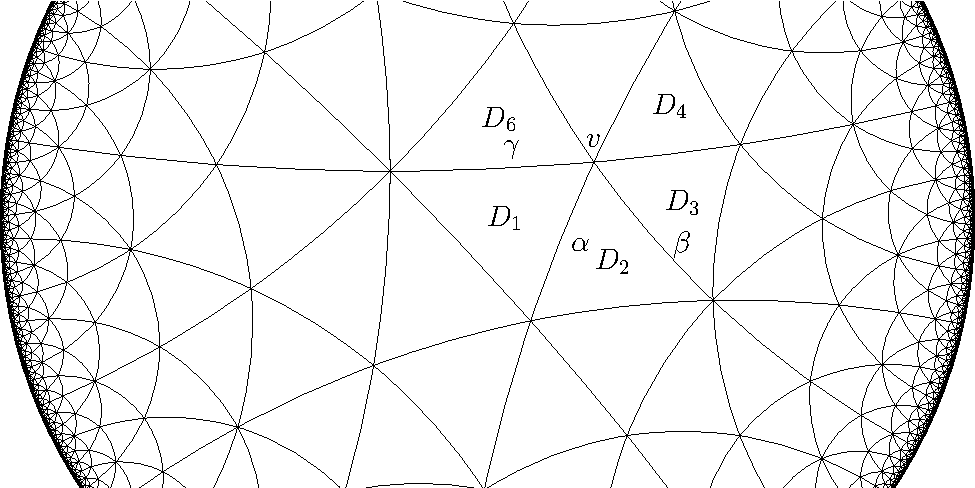
\includegraphics{diagrams/deg6433f2.pdf}
		\caption{Case: $|\st(v)|=6$}
	\end{figure}

	
	Now suppose $|\st(v)|=8.$ Then we will use the same labeling scheme as before except there will be $8$ chambers, and each positive root will contain exactly 4 consecutive chambers from $\st(v).$ The same logic as before will still tell us that $\gamma$ will contain exactly the chambers $D_1,D_2,D_3,D_4.$ Our first claim is that $D_2=\proj_v(C).$

	We know that $\proj_v(C)$ must lie in any positive root through $v$ and thus it can only be $D_1,D_2,D_3,D_4.$ We also know it is the chamber $A$ in $\st(v)$ which minimizes $d(A,C).$ Since $d(D_1,C)>d(D_2,C)$ we know that $D_1$ cannot be the projection. By a similar argument as before we know that $D_4$ borders $\gamma$ and thus $d(D_4,C)\ge d(D_1,C)$ by our choice of $D_1.$ Thus $D_4$ cannot be the projection. Finally, if $D_3$ were the projection then $d(D_4,C)=d(D_3,C)+1<d(D_3,C)+2=d(D_1,C)$ which is also a contradiction and thus $D_2=\proj_v(C).$

	Let $\alpha$ be the positive root separating $D_1$ and $D_2,$ $\beta$ the positive root separating $D_2$ and $D_3$ and $\delta$ the positive root separating $D_3$ and $D_4.$ Recall that $\gamma$ is the positive root separating $D_8$ and $D_1$ as well as $D_4$ and $D_5.$ We know that $D_2$ borders $\alpha$ and $\beta$ with $d(D_2,C)=d(D_1,C)-1=n-1$ and thus $U_\alpha,U_\beta\subset U_{n-1}.$ We also know that $D_2$ lies in all positive roots through $v$ by convexity so $D_2\in \alpha,\beta,\gamma,\delta.$ Since $D_2$ is bordered by $\alpha$ and $\beta$ we also know that $\alpha$ and $\beta$ are the simple roots at $v.$
	\begin{figure}[h]
		\label{fig:334deg8}
	\begin{center}
		%\import{diagrams/}{deg8433f2}
		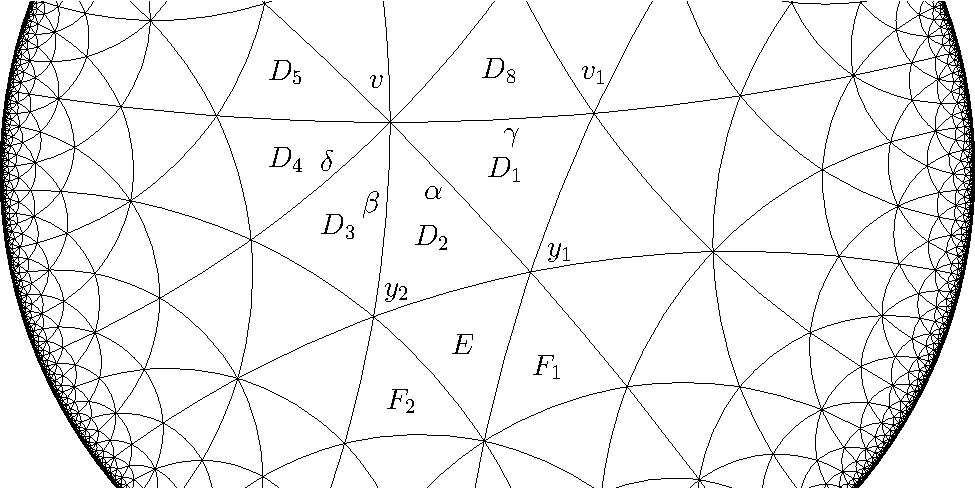
\includegraphics{diagrams/deg8433f2.pdf}
	\end{center}
	\caption{Case: $|\st(v)=8|$}
\end{figure}

Let $E$ be the third chamber adjacent to $D_2.$ Every chamber must have an adjacent chamber which is closer to $C$ and thus we have $d(E,C)<d(D_2,C).$ We can check that $d(E,C)=d(D_1,C)-2\ge 1$ by our choice of $\gamma$ and thus $E$ is not the fundamental chamber $C.$ We know that $D_1$ and $D_2$ share two vertices, and $D_2$ and $E$ share two vertices, so necessarily we have that $D_1,D_2,$ and $E$ must share at least one, and thus exactly one vertex, call it $y_1.$ By a similar argument, the chambers $D_3,D_2,$ and $E$ will also share a vertex $y_2.$ Let $F_1$ be the other chamber adjacent to $E$ that has $y_1$ as a vertex, and let $F_2$ be the other chamber adjacent to $E$ that has $y_2$ as a vertex. Note that $|\st(y_1)|=|\st(y_2)|=6$ since $v$ is the other vertex of $D_2.$ The appropriate labeling can be seen in Figure \ref{fig:334deg8}, and the given diagram is unique up to a mirror image flip, which does not affect any of the following arguments. The labeling of these chambers could have simply been defined by the diagram, but the previous explanation seeks to convince the reader that no choices have been made and this diagram is unique.

Since $d(E,C)<d(D_2,C)<d(D_1,C)$ we know that there is some minimal gallery from $D_1$ to $C$ which passes through $E.$ If we fix such a minimal gallery we can see that it must pass through either $F_1$ or $F_2.$ First suppose that it passes through $F_1.$ Then $d(F_1,C)=d(D_1,C)-3$ and so $F_1$ and $D_1$ are distance 3 from one another. Since they are both in $\st(y_1),$ this means that $D_1$ and $F_1$ are opposite in $\st(y_1).$ Then there is another minimal gallery from $D_1$ to $F_1$ which does not pass through $D_2$ and can also be extended to a minimal gallery from $D_1$ to $C.$ Let $G_1$ be the chamber adjacent to $D_1$ in this new minimal gallery. Then $D_1$ and $G_1$ have exactly two vertices in common, on of which is $y_1,$ and the other cannot be $v$ as this would imply $G_1=D_2$ which contradicts our assumption. Let $v_1$ be the common vertex which is not $y_1.$ We assumed that $v$ was the unique vertex shared by $D_1$ and $D_2$ which lies on $\partial \gamma.$ Since $y_1$ is also shared by $D_1$ and $D_2$ this means that $y_1$ does not lie on $\partial \gamma.$ We assumed that $D_1$ has a panel on $\partial \gamma$ and thus it has two vertices on $\partial \gamma$ which means $v_1$ must lie on $\partial \gamma.$

Now we have the following situation. We still know that $D_1$ borders $\gamma$ with $d(\gamma,C)=d(D_1,C)$ and $G_1$ is an adjacent chamber such that $d(G_1,C)<d(D_1,C).$ We know that $v_1$ is a common vertex which lies on $\partial\gamma$ and thus it is the only common vertex which lies on $\partial\gamma.$ Finally, $v$ is the uniqe vertex of $D_1$ with 8 chambers in its star. Thus $|st(v_1)|=6.$ Now we may apply the $|\st(v)|=6$ case with $G_1$ as our new choice of $D_2$ and $v_1$ the new $v.$ This shows that $U_\gamma\subset U_{n-1}$ as desired.

Now suppose the fixed minimal gallery from before passes through $F_2.$ The arguments made here will be very similar to those made in the previous paragraphs, as there is an obvious symmetry in the Coxeter complex, but we will explain the arguments again, if a little more briefly. There is also a minimal gallery from $D_3$ to $C$ which passes through $F_2$ as well. But then $d(F_2,C)=d(D_3,C)-3$ which means $F_2$ and $D_3$ are opposite in $\st(y_2).$ Then there is another minimal gallery in $\st(y_2)$ from $D_3\to F_2$ which does not pass through $D_2.$ Let $G_2$ be the chamber adjacent to $D_3$ in this new minimal gallery. Then $G_2$ and $D_3$ will have two vertices in common and one of them will be $y_2.$ Let $v_2$ be the other vertex in common. Then $v_2$ must lie on $\partial \delta$ since $y_2$ is the only vertex of $D_3$ which does not lie on $\partial \delta.$ We also know that $|\st(v_2)|=6$ as $v$ is the only vertex of $D_3$ with $|\st(v)|=12.$

Since $D_3$ borders $\delta$ we know that $d(\delta,C)\le n.$ If $d(\delta,C)<n$ then $U_{\delta}\subset U_{n-1}.$ If $d(\delta,C)=n$ then we have the following situation: $D_3$ is a chamber which borders $\delta$ and $d(\delta,C)=d(D_3,C).$ Furthermore, $G_2$ is a chamber adjacent to $D_3$ with $d(G_2,C)=d(D_3,C)-1.$ The unique, common vertex which lies on $\partial\delta$ is $v_2$ and it has $|\st(v_2)|=6.$ Thus we can apply that $|st(v)=6|$ case to see that $U_\delta\subset U_{n-1}.$ But $U_v=\langle U_\alpha,U_\beta,U_\delta\rangle$ and thus $U_\gamma\subset U_{n-1}$ as desired.

Now we have shown that $U_\gamma \subset U_{n-1}$ in any case, and since the choice of $\gamma$ such that $d(\gamma,C)=n>2$ was arbitrary, we know that $U_n\subset U_{n-1}$ for $n>2$ as desired.
\end{proof}

\begin{cor}
	\label{cor:334f2fg}
	Suppose $(G,(U_\alpha)_{\alpha\in \Phi},T)$ is an RGD system of type $(W,S)$ with $S=\{s,t,u\}.$ If $m(s,t)=m(s,u)=3$ and $U_x\cong C_2(2)$ for the vertex $x$ of $C$ of type $s$ then $U_+$ is finitely generated.
\end{cor}

\subsection{Case: 336 over $\F{3}$}

Now we consider the last exceptional case. In this section we assume $(G,(U_\alpha)_{\alpha\in \Phi},T)$ is an RGD system of type $(W,S)$ with $S=\{s,t,u\}.$ Assume that $m(s,t)=m(s,u)=3$ and $U_x\cong G_2(3)$ where $x$ is the vertex of the fundamental chamber $C$ of type $s.$ We will show that $U_+$ is finitely generated.

%While the geometry will be slightly more complicated, the strategy in this section will be the same as in the previous section. 
%\begin{theorem}
%	\label{thm:336f3fg}
%	Let $(G,(U_\alpha)_{\alpha\in \Phi},T)$ of type $(W,S)$ as above. If $x$ is the vertex of $C$ of type $s$ and $U_x\cong C_2(2)$ then $U_n\subset U_{n-1}$ for all $n>2$ where $U_n=\langle U_\gamma|d(\gamma,C)\le n\rangle.$
%\end{theorem}
%\begin{proof}
%	Let $\gamma$ be a positive root of $\Sigma$ with $d(\gamma,C)=n>2.$ We must show that $U_\gamma \subset U_{n-1}.$ Let $D$ be a chamber which borders $\gamma$ such that $d(\gamma,C)=d(D,C).$ Since $d(\gamma,C)=d(D,C)>2$ we know that $D\neq C$ and thus there is a chamber adjacent to $D$ which is closer to $C.$ Let $D'$ be a chamber adjacent to $D$ which is closer to $C.$ Then $D$ and $D'$ have two vertices in common, and $D$ has two vertices on $\partial \gamma,$ so there is a vertex $v$ in common between $D$ and $D'$ which lies on $\partial \gamma.$ Now there are two possibilites for $v,$ either $|\st(v)|=6$ or $|\st(v)|=12.$
%
%	First consider when $|\st(v)|=6.$ Let $\alpha_1,\alpha_2,\alpha_3$ be a standard labeling of the positive roots through $v$ and let $E=\proj_v(C).$ Since $\gamma$ is a positive root through $v$ we know that $\gamma=\alpha_i$ for some $1\le i\le 3.$ By the properties of projections, we know that $E$ is the chamber in $\st(v)$ which is closest to $C.$ By construction, the chamber $D'$ lies in $\st(v)$ and has $d(D',C)<d(D,C).$ Thus $D\neq E.$ Thus $d(E,C)<d(D,C).$ We know that $\alpha_1$ and $\alpha_3$ border $E$ and thus $d(\alpha_1,C),d(\alpha_3,C)\le d(E,C)<n$ which means that $U_{\alpha_1},U_{\alpha_3}\subset U_{n-1}.$ But $U_v=\langle U_{\alpha_1},U_{\alpha_3}\rangle$ since $U_v$ cannot be an exceptional rank 2 group, and thus $U_v\subset U_{n-1}$ as well. Thus $U_\gamma \subset U_{n-1}$ as desired.
%
%	Now suppose that $|\st(v)|=12.$ Let $\alpha_1,\dots,\alpha_6$ be a standard labeling of the positive roots through $v$ and let $E=\proj_{v}(C)$ as before. As before, we know that $\gamma=\alpha_i$ for some $i$ and $D\neq E.$ Since $\alpha_1$ and $\alpha_6$ will border $E$ we know that $U_{\alpha_1},U_{\alpha_6}\subset U_{n-1}.$ Since we can reverse the order of the standard labeling, assume that $\gamma=\alpha_i$ for some $1\le i\le 3.$ First suppose that $\gamma=\alpha_1.$ Then we know that $D\in \alpha_1$ with a panel on $\alpha_1$ by definition, and we also know that $E\in \alpha_1$ with a panel on $\alpha_1$ by the properties of projections. Since $E\neq D$ and they both have a panel on $\partial \alpha_1$ we know that $d(D,E)=5$ and thus $d(D,C)=d(E,C)+5.$ But there is a chamber $D''$ adjacent to $E$ along $\partial\alpha_1$ which would imply $d(D'',C)=d(E,C)+1.$ But then $D''$ border $\gamma$ and $d(D'',C)<d(D,C)$ which is a contradiction of our choice of $D.$ Thus $\gamma$ cannot be $\alpha_1.$ 
%
%	Now suppose $\gamma=\alpha_3.$ 
%
%\end{proof}
Recall from the previous section that for any positive roots $\gamma,$ we define $d(\gamma,C)$ to be the minimal distance between $C$ and any chamber with a panel on $\partial\gamma.$ We then define $U_k$ to be the subgroup of $U_+$ generated by all $U_\alpha$ with $\alpha\in \Phi_+$ and $d(\alpha,C)\le k.$

\end{document}
